\documentclass{report}
\usepackage[utf8]{inputenc}

\title{Relatório de Instalação do Windows 3.1}
\author{Acadêmico: Felipe Helfensteler Beskow RA: 1581201}

\date{2019/02}

\usepackage[portuguese]{babel}
\usepackage{natbib}
\usepackage{graphicx}
\usepackage{hyperref}

\hypersetup{
    colorlinks=false
}
\urlstyle{same}

\begin{document}

\maketitle

\chapter{Introdução}
O Windows 3.1 simplesmente revolucionou o mundo da IBM-PC com seu modo gráfico e programação multitarefas. A Microsoft, que começou no mercado de Sistemas Operacionais com um simples sistema mono tarefa, veio com o Windows prometendo dominar o mercado. \\
Para rodas o Windows havia alguns pré-requisitos, um deles era ter o MS-DOS instalado.

\chapter{Materiais e Métodos}

\section{Oracle VM VirtualBox}
Para poder rodar o sistema operacional foi usado o software Oracle VM Virtual simulando um computador virtual que podemos configurar de maneira compatível com o MS-DOS e Windows 3.1.\\
Ele está disponível para download através do site: \url{https://www.virtualbox.org/}.

\section{Imagem do MS-DOS}
MS-DOS, acrônico \textit{Microsoft Disk Operating System}, é um sistema operacional mono tarefa comprado pela Microsoft para o IBM PC. Ele foi usado de base para criar as primeiras versões do Windows, até a Microsoft criar o Windows NT.

\section{Imagem do Windows 3.1}
O Windows surgiu como uma forma de tornar o MS-DOS mais produtivo, de maneira que pudesse utilizar vários programas ao mesmo tempo. Ele integrava uma interface gráfica que facilitava ao usuário a interação com o computador.

\chapter{Preparar o Ambiente}

Em primeiro de tudo foi necessário criar uma máquina virtual no VirtualBox:
\begin{figure}[h]
\centering
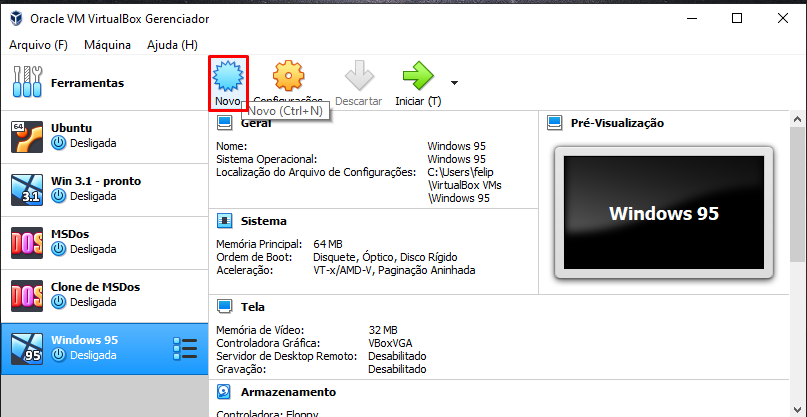
\includegraphics[width=\textwidth]{Screenshot_1.png}
\caption{Criar máquina virtual}
\label{fig:1}
\end{figure}

\begin{figure}
\centering
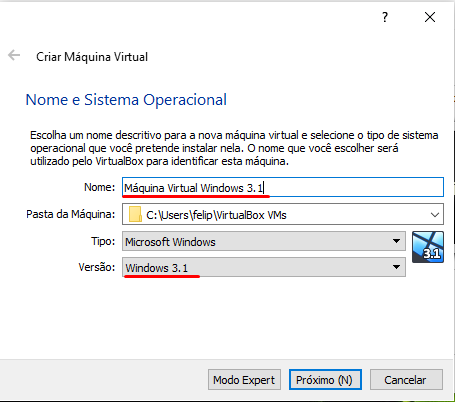
\includegraphics[width=\textwidth]{Screenshot_2.png}
\caption{Criar máquina virtual}
\label{fig:2}
\end{figure}

\begin{figure}
\centering
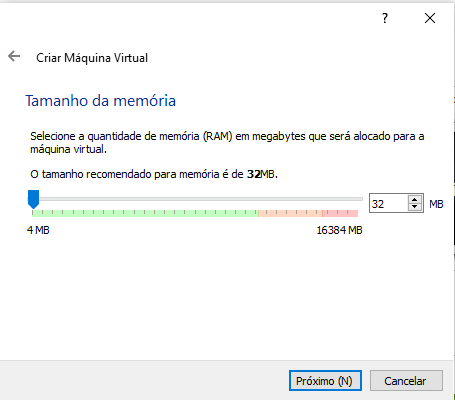
\includegraphics[width=\textwidth]{Screenshot_3.png}
\caption{Criar máquina virtual}
\label{fig:3}
\end{figure}

\begin{figure}
\centering
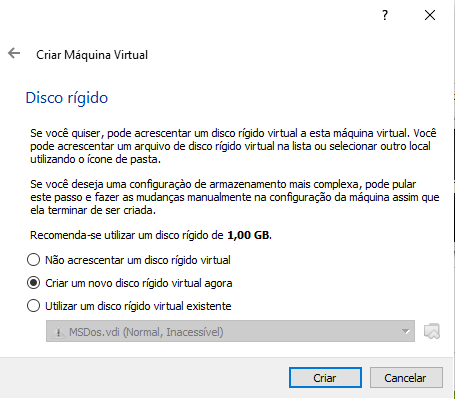
\includegraphics[width=\textwidth]{Screenshot_4.png}
\caption{Criar máquina virtual}
\label{fig:4}
\end{figure}

\begin{figure}
\centering
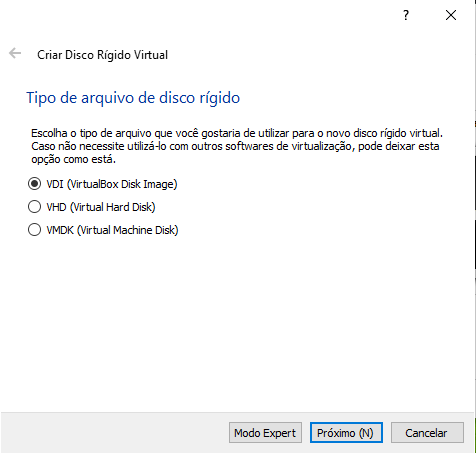
\includegraphics[width=\textwidth]{Screenshot_5.png}
\caption{Criar máquina virtual}
\label{fig:5}
\end{figure}

\begin{figure}
\centering
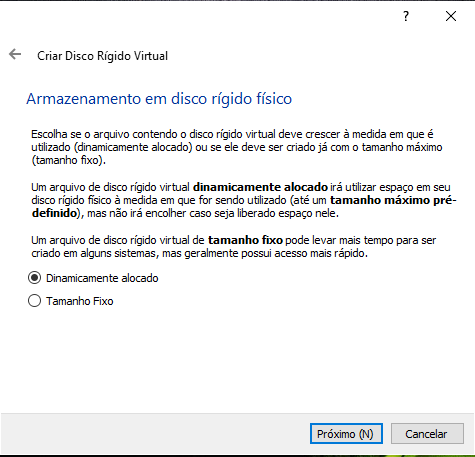
\includegraphics[width=\textwidth]{Screenshot_6.png}
\caption{Criar máquina virtual}
\label{fig:6}
\end{figure}

\begin{figure}
\centering
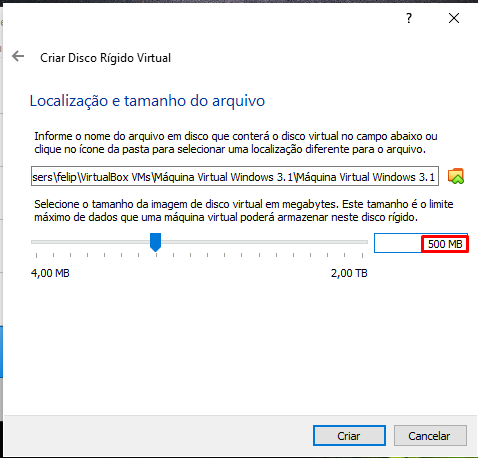
\includegraphics[width=\textwidth]{Screenshot_7.png}
\caption{Criar máquina virtual}
\label{fig:7}
\end{figure}
\newpage
\begin{figure}
\centering
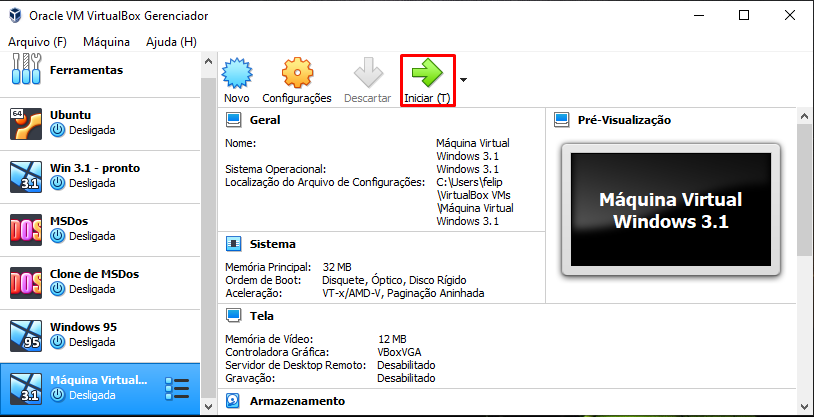
\includegraphics[width=\textwidth]{Screenshot_8.png}
\caption{Criar máquina virtual}
\label{fig:8}
\end{figure}

Após esses passos começamos instalando o MS-DOS:

\begin{figure}
\centering
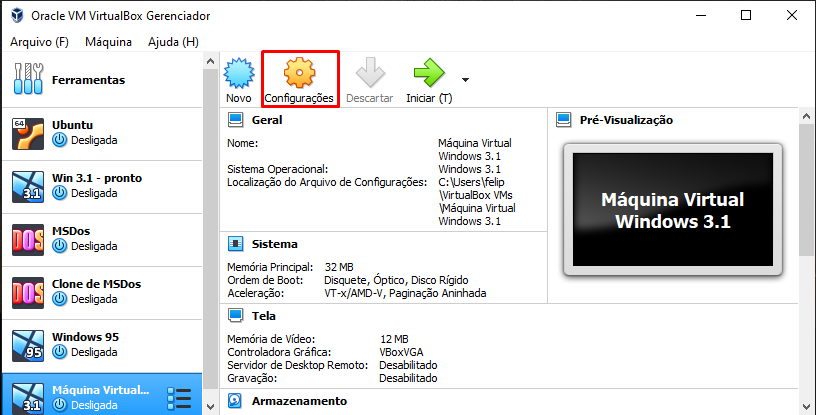
\includegraphics[width=\textwidth]{Screenshot_9.png}
\caption{Instalar MS-DOS}
\label{fig:9}
\end{figure}

\begin{figure}
\centering
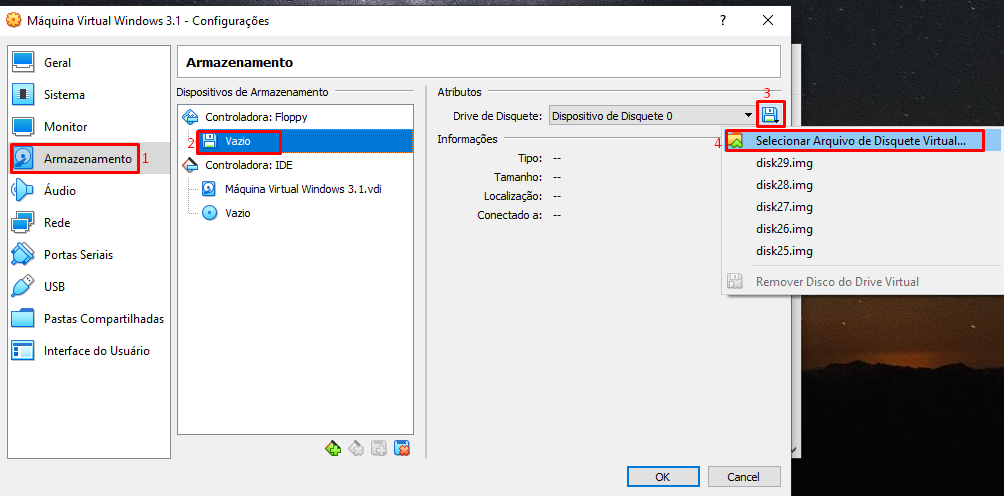
\includegraphics[width=\textwidth]{Screenshot_10.png}
\caption{Instalar MS-DOS}
\label{fig:10}
\end{figure}

\begin{figure}
\centering
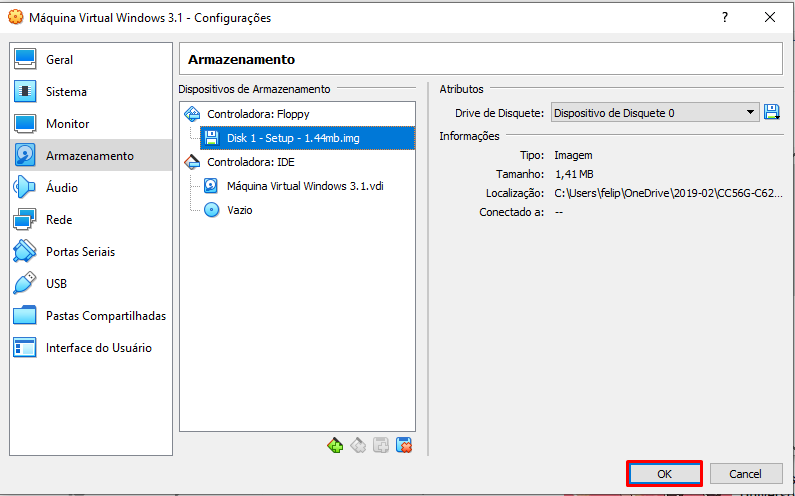
\includegraphics[width=\textwidth]{Screenshot_11.png}
\caption{Instalar MS-DOS}
\label{fig:11}
\end{figure}

\begin{figure}
\centering
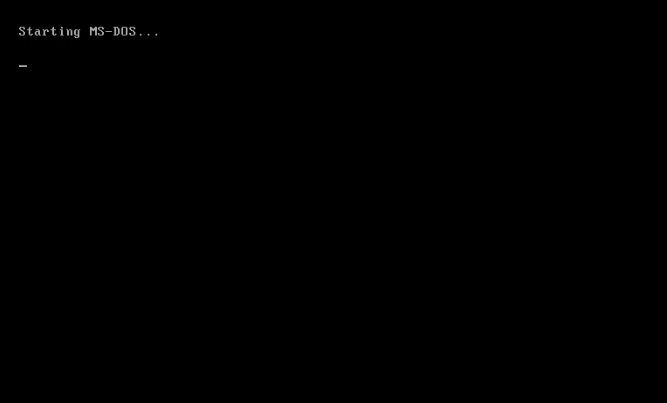
\includegraphics[width=\textwidth]{Screenshot_12.png}
\caption{Instalar MS-DOS}
\label{fig:12}
\end{figure}

\begin{figure}
\centering
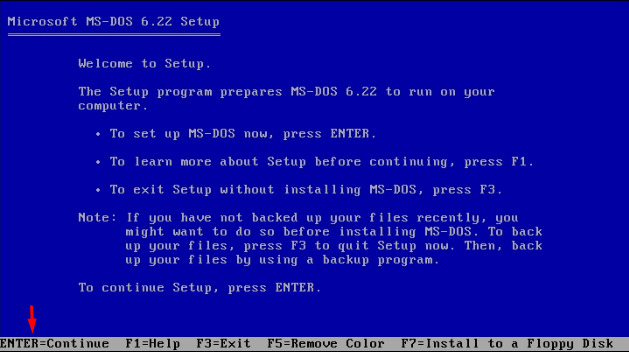
\includegraphics[width=\textwidth]{Screenshot_13.png}
\caption{Instalar MS-DOS}
\label{fig:13}
\end{figure}

\begin{figure}
\centering
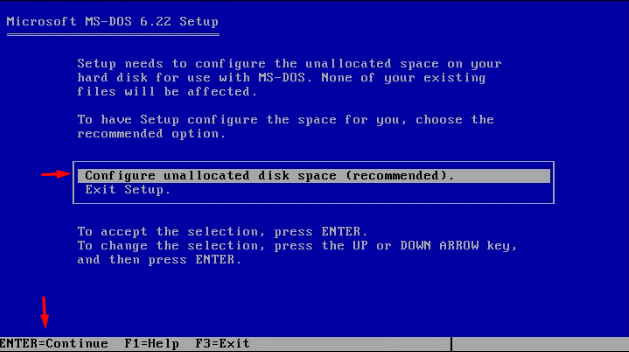
\includegraphics[width=\textwidth]{Screenshot_14.png}
\caption{Instalar MS-DOS}
\label{fig:14}
\end{figure}

\begin{figure}
\centering
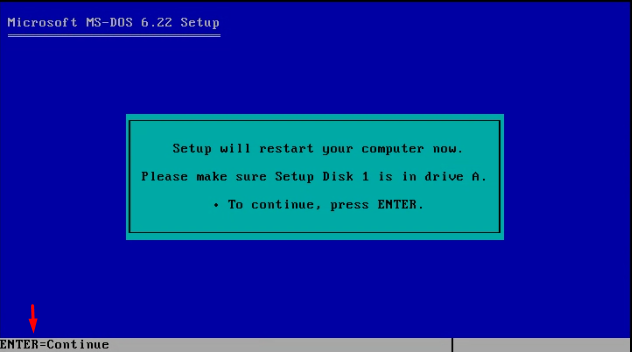
\includegraphics[width=\textwidth]{Screenshot_15.png}
\caption{Instalar MS-DOS}
\label{fig:15}
\end{figure}

\begin{figure}
\centering
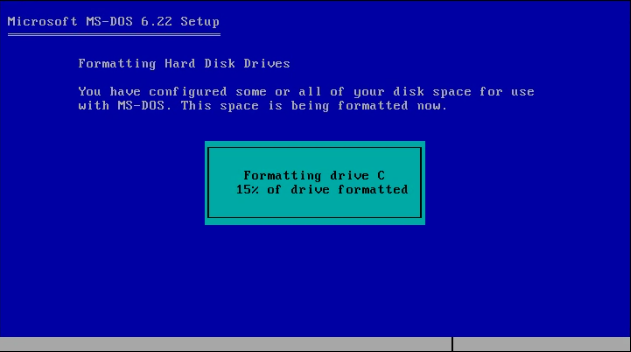
\includegraphics[width=\textwidth]{Screenshot_16.png}
\caption{Instalar MS-DOS}
\label{fig:16}
\end{figure}

\begin{figure}
\centering
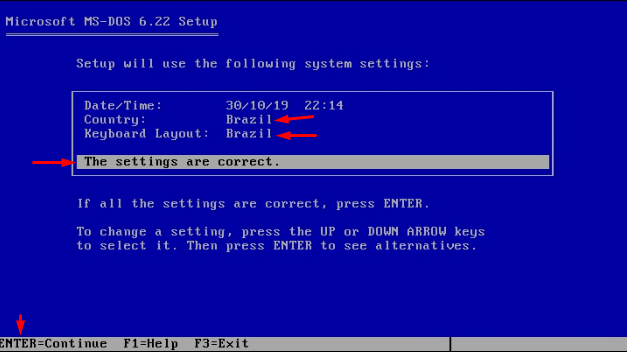
\includegraphics[width=\textwidth]{Screenshot_17.png}
\caption{Instalar MS-DOS}
\label{fig:17}
\end{figure}

\begin{figure}
\centering
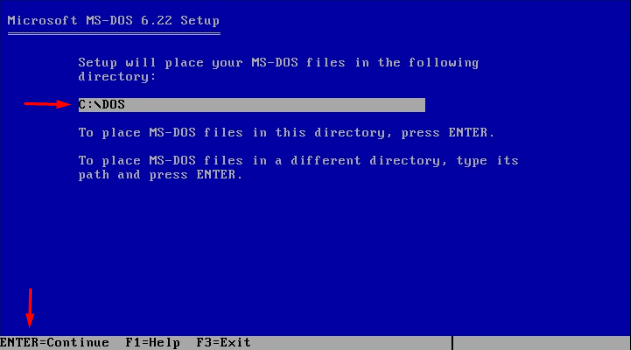
\includegraphics[width=\textwidth]{Screenshot_18.png}
\caption{Instalar MS-DOS}
\label{fig:18}
\end{figure}

\begin{figure}
\centering
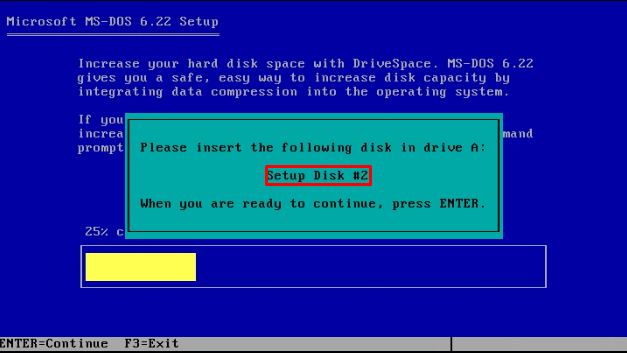
\includegraphics[width=\textwidth]{Screenshot_19.png}
\caption{Instalar MS-DOS}
\label{fig:19}
\end{figure}

\newpage
Após isso, é só ir trocando os disquetes até que a instalação do MS-DOS esteja completa.

\begin{figure}
\centering
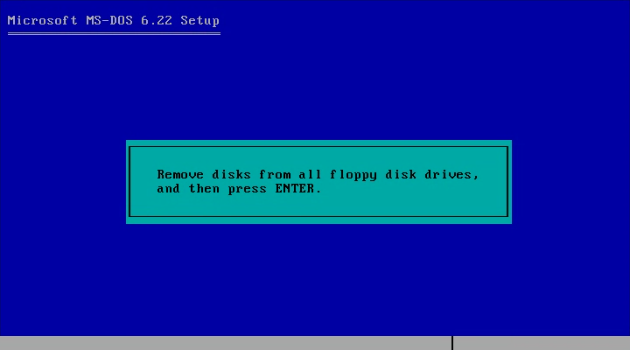
\includegraphics[width=\textwidth]{Screenshot_20.png}
\caption{Instalar MS-DOS}
\label{fig:20}
\end{figure}

\newpage
Agora reiniciar o computador, o MS-DOS estará instalado, pronto para receber o Windows.


\chapter{Instalar o Windows 3.1}

Feita a instalação do MS-DOS, iremos começar a instalação do Windows 3.1:

\begin{figure}
\centering
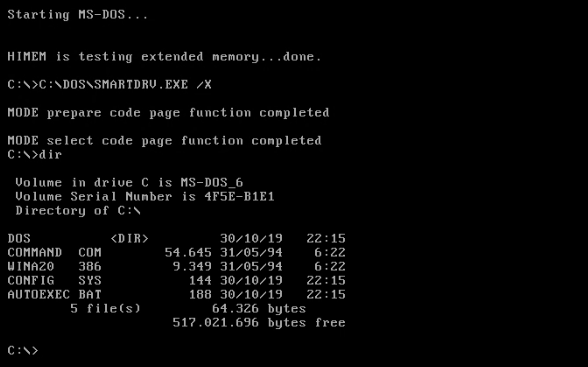
\includegraphics[width=\textwidth]{Screenshot_21.png}
\caption{Instalar Windows 3.1}
\label{fig:21}
\end{figure}

\begin{figure}
\centering
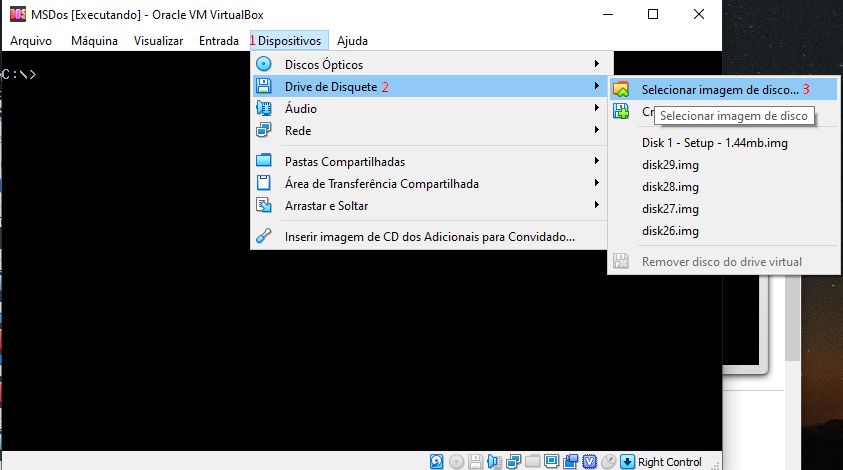
\includegraphics[width=\textwidth]{Screenshot_22.png}
\caption{Instalar Windows 3.1}
\label{fig:22}
\end{figure}

\begin{figure}
\centering
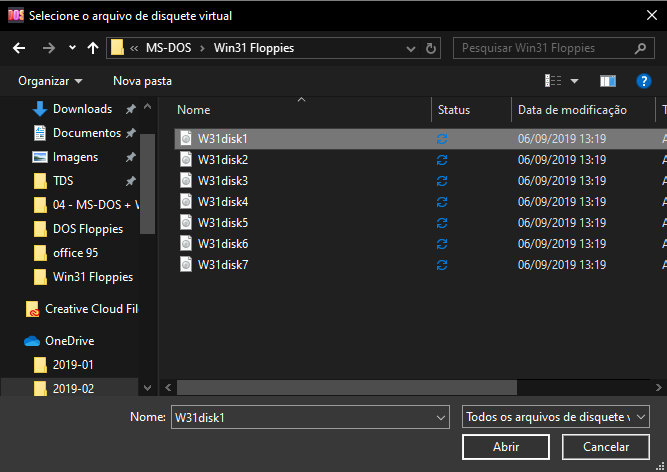
\includegraphics[width=\textwidth]{Screenshot_23.png}
\caption{Instalar Windows 3.1}
\label{fig:23}
\end{figure}

\begin{figure}
\centering
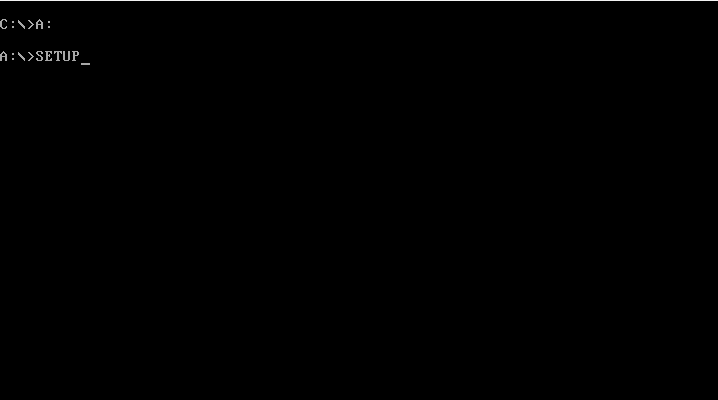
\includegraphics[width=\textwidth]{Screenshot_24.png}
\caption{Instalar Windows 3.1}
\label{fig:24}
\end{figure}

\begin{figure}
\centering
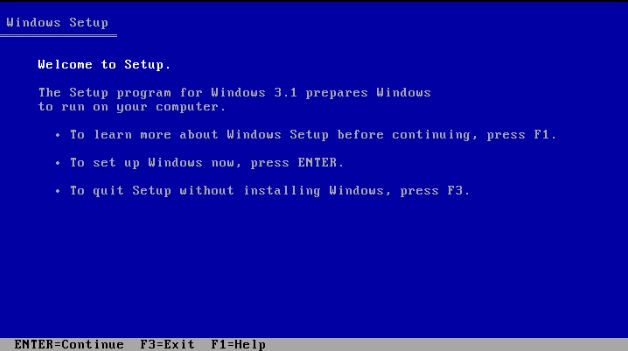
\includegraphics[width=\textwidth]{Screenshot_25.png}
\caption{Instalar Windows 3.1}
\label{fig:25}
\end{figure}

\begin{figure}
\centering
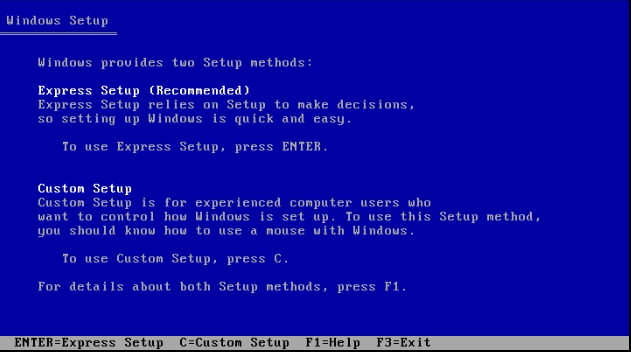
\includegraphics[width=\textwidth]{Screenshot_26.png}
\caption{Instalar Windows 3.1}
\label{fig:26}
\end{figure}

\begin{figure}
\centering
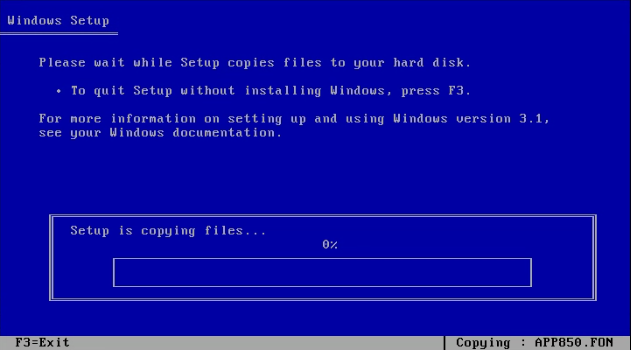
\includegraphics[width=\textwidth]{Screenshot_27.png}
\caption{Instalar Windows 3.1}
\label{fig:27}
\end{figure}

\begin{figure}
\centering
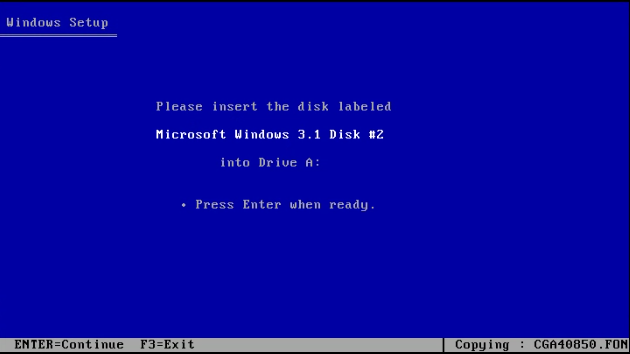
\includegraphics[width=\textwidth]{Screenshot_28.png}
\caption{Instalar Windows 3.1}
\label{fig:28}
\end{figure}

\begin{figure}
\centering
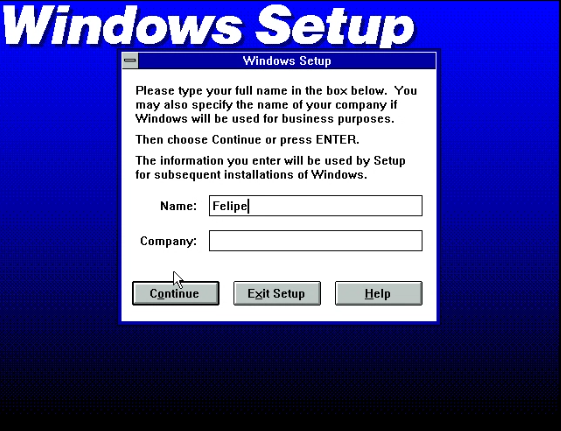
\includegraphics[width=\textwidth]{Screenshot_29.png}
\caption{Instalar Windows 3.1}
\label{fig:29}
\end{figure}

\begin{figure}
\centering
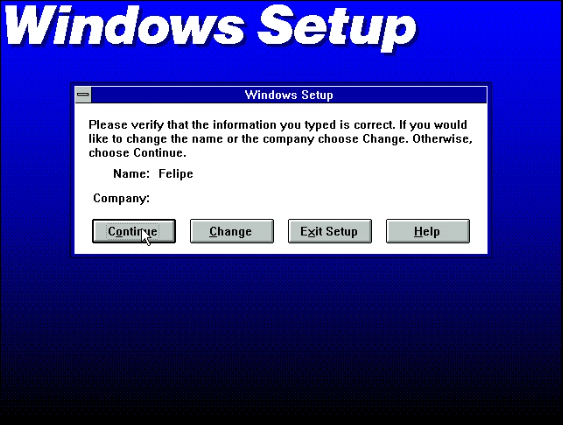
\includegraphics[width=\textwidth]{Screenshot_30.png}
\caption{Instalar Windows 3.1}
\label{fig:30}
\end{figure}

\begin{figure}
\centering
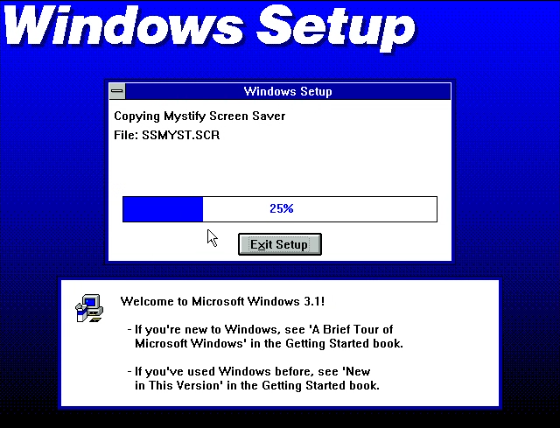
\includegraphics[width=\textwidth]{Screenshot_31.png}
\caption{Instalar Windows 3.1}
\label{fig:31}
\end{figure}

\begin{figure}
\centering
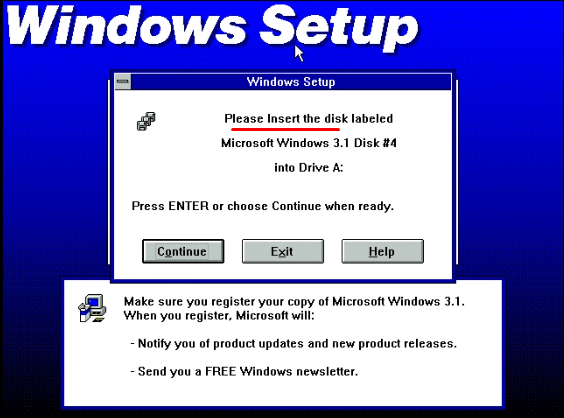
\includegraphics[width=\textwidth]{Screenshot_32.png}
\caption{Instalar Windows 3.1}
\label{fig:32}
\end{figure}

\begin{figure}
\centering
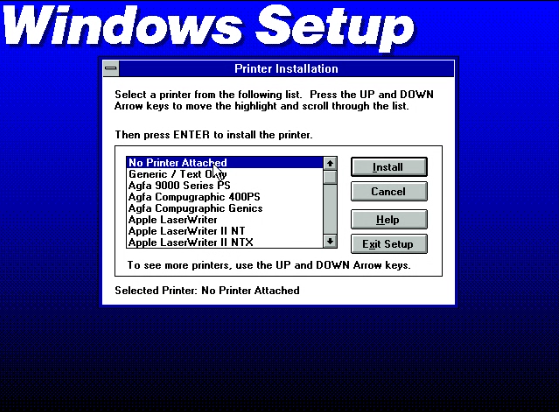
\includegraphics[width=\textwidth]{Screenshot_33.png}
\caption{Instalar Windows 3.1}
\label{fig:33}
\end{figure}

\begin{figure}
\centering
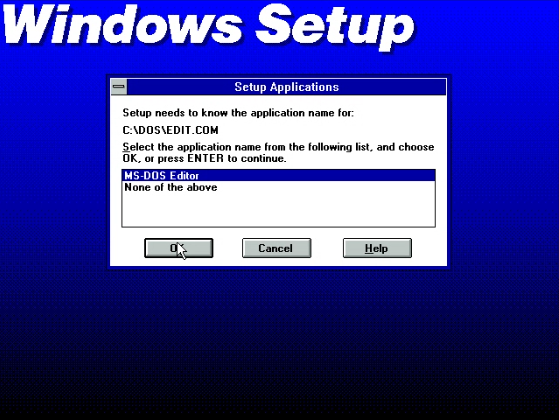
\includegraphics[width=\textwidth]{Screenshot_34.png}
\caption{Instalar Windows 3.1}
\label{fig:34}
\end{figure}

\begin{figure}
\centering
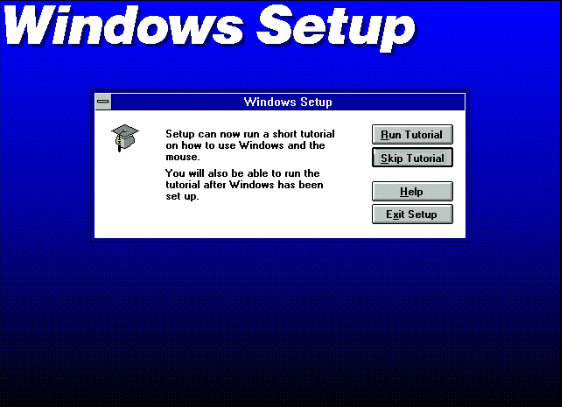
\includegraphics[width=\textwidth]{Screenshot_35.png}
\caption{Instalar Windows 3.1}
\label{fig:35}
\end{figure}

\begin{figure}
\centering
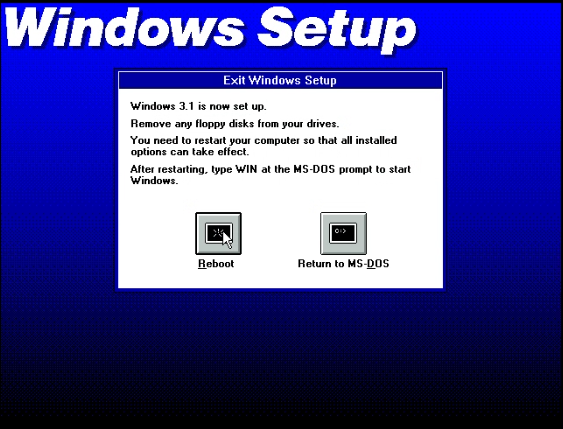
\includegraphics[width=\textwidth]{Screenshot_36.png}
\caption{Instalar Windows 3.1}
\label{fig:36}
\end{figure}

\begin{figure}
\centering
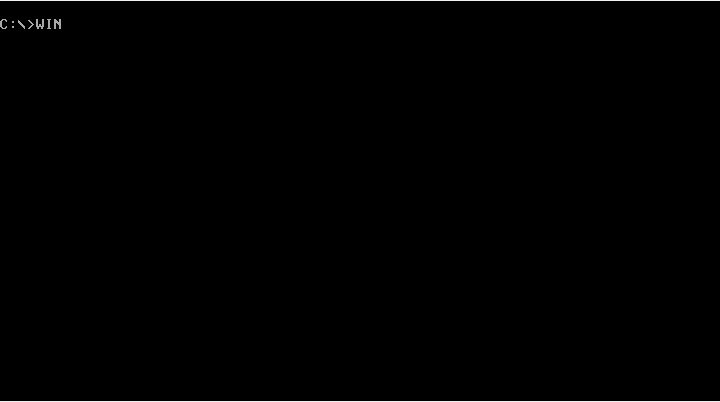
\includegraphics[width=\textwidth]{Screenshot_37.png}
\caption{Instalar Windows 3.1}
\label{fig:37}
\end{figure}

\begin{figure}
\centering
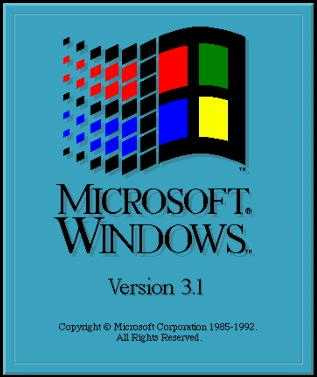
\includegraphics[width=\textwidth]{Screenshot_38.png}
\caption{Instalar Windows 3.1}
\label{fig:38}
\end{figure}

\begin{figure}
\centering
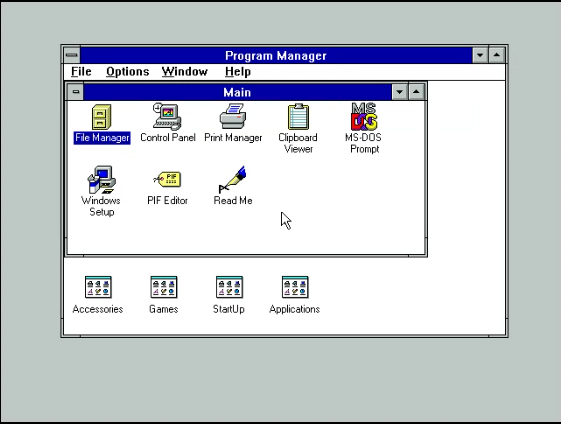
\includegraphics[width=\textwidth]{Screenshot_39.png}
\caption{Instalar Windows 3.1}
\label{fig:39}
\end{figure}

\chapter{Conclusões}

Instalar o Windows 3.1 trouxe uma perspectiva do passado dos computadores e sistemas operacionais modernos. Apesar de o MS-DOS não chegar aos pés do Unix, ele conquistou mais consumidores.

\begin{thebibliography}{9}
\bibitem{windows3}
Windows 3.x. Wikipédia, a enciclopédia livre., 2019. Disponível em: https://pt.wikipedia.org/wiki/Windows\underline{ }3.x. Acesso em: 30 out. 2019.
\bibitem{virtualbox}
VirtualBox. Disponível em: https://www.virtualbox.org/. Acesso em: 30 out. 2019.
\bibitem{msdos}
MS-DOS. Wikipédia, a enciclopédia livre., 2019. Disponível em: https://pt.wikipedia.org/wiki/MS-DOS. Acesso em: 30 out. 2019.
\end{thebibliography}
\end{document}
